% !TeX root = ../../main.tex
% chktex-file 13
\section{Technology Stack}\label{section:technology-stack}

Since most of the existing software for \ac{UBII} was written in \acf{JS}\footnote{\ac{JS} is a just-in-time compiled scripting language, widely used in web technology. It is a dynamic prototype-based language, which supports object-orientated programming.} using a web-based architecture, I decided to adapt this approach for my application. This has the major advantage of platform independence. Most modern devices can run web-based software, which means they can also run my application. Also the application is served by a web server, which means the user does not have to install the software onto his device.

\begin{figure}[htpb]
  \centering
  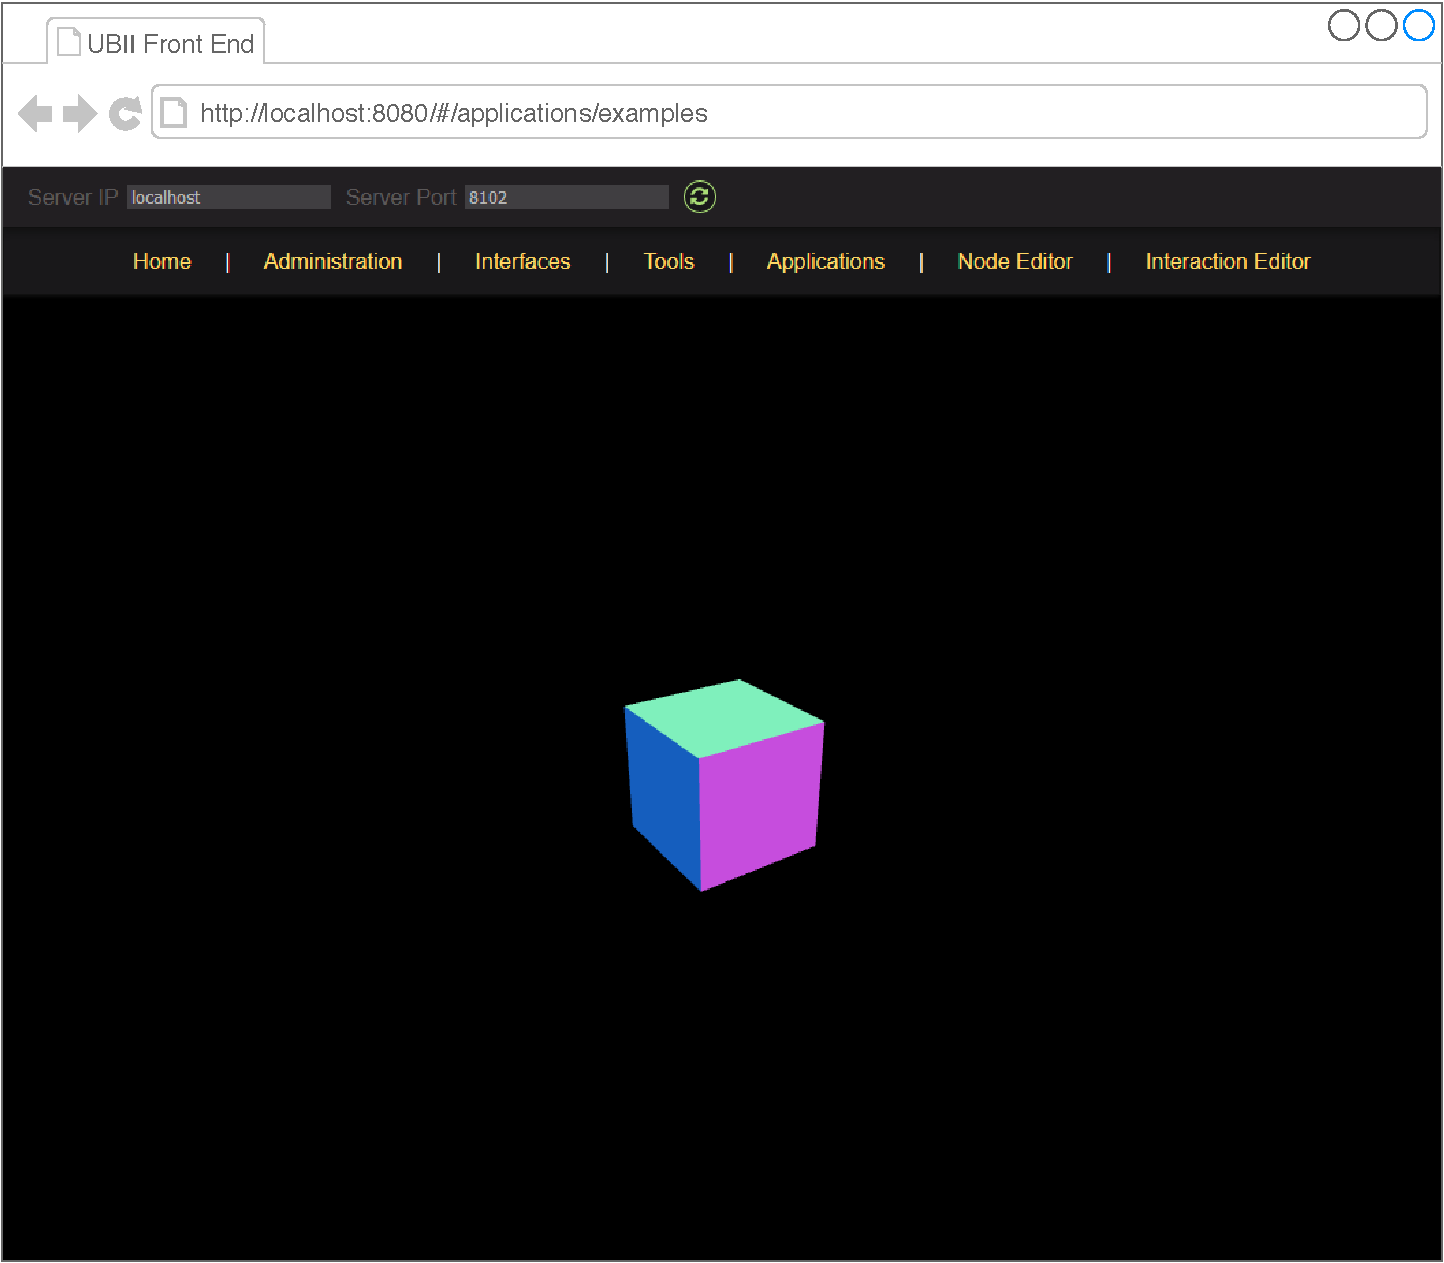
\includegraphics[width=12cm]{figures/ubii_front_end.pdf}
  \caption[Screenshot of the UBII front end]{A screenshot of the UBII front end rendering a 3D cube.}\label{fig:ubii-front-end}
\end{figure}

A web interface with some \ac{UBII} content (the \ac{UBII} front end), demos and debugging tools was already written\footnote{The front end was developed by Sandro Weber, Daniel Dyrda and me.}, so I included my experiments in this application as well. The technology stack of the front end was built with the following technologies:
\begin{description}
  \item[Web APIs] are \acfp{API} available in modern web browsers to provide access to functionality or data outside the browser. The WebAPI is an additional layer of abstraction of the \acp{API} of an operating system. While this has the advantage that the API is the same on every device, this also prevents the access to the raw sensor data\footnote{The specification is available on \href{https://w3c.github.io/deviceorientation/}{www.w3c.github.io/deviceorientation}}. In this thesis the WebVR \ac{API} and the device orientation \ac{API} were used. The former enables to render to external \ac{VR} headsets. The latter gives access to the data of the \acf{IMU}\footnote{An IMU is an electronic component which is part of most smart phones and allows to measure force, angular rate and magnetic field.}.
  \item[Vue.js]\footnote{Vue.js: Website: \href{https://vuejs.org/}{www.vuejs.org}, Source~code: \href{https://github.com/vuejs/vue}{www.github.com/vuejs/vue}} is a modern open source \acl{JS} web framework\footnote{A web framework is a software framework which provides a standard way to build web applications. It comes with tools and libraries to automate and make the development of web applications easier.}~\cite{EvanYou.2019}. Being released in 2014 and developed by Evan You, it is a relatively young framework~\cite[17]{Koetsier.2016}. But it quickly gained traction and is quite popular now~\cite[12\psq]{Koetsier.2016}.
  Packages like Vue.js itself, Vue.js plugins and other \acl{JS} libraries are managed using the package manager npm~\footnote{\enquote{NPM} stands for \enquote{Node Package Manager} and is also used in the~\ac{UBII} server itself. Website: \href{https://www.npmjs.com/}{www.npmjs.com}}.
  \item[Three.js]\footnote{Three.js: Website: \href{https://threejs.org/}{www.threejs.org}, Source~code: \href{https://github.com/mrdoob/three.js/}{www.github.com/mrdoob/three.js}} is a lightweight open source library which utilizes WebGL to render \ac{3D} computer graphics~\cite{RicardoCabello.2019}. It can be used to render scenes to the display as well as to a VR headset using WebVR. This high-level library comes with a lot of features, similar to a game engine, like scenes, effects, lights, animation, geometrie and much more.
  \item[UBII Client] is an \acl{JS} client for the \ac{UBII} system. It abstracts the protocol and provides high-level functions to register devices as well as send and receive topic data. The UBII system uses \acf{Protobuf}\footnote{Protobuf is a mechanism to serialize data. The data is defined in a platform-neutral language, which compiles as library to all commonly used programming languages~\cite{GoogleLLC.2019}. Website: \href{https://developers.google.com/protocol-buffers/}{www.developers.google.com/protocol-buffers/}} to serialize the data.
\end{description}

Figure~\ref{fig:ubii-front-end} displays an test view, which uses Vue.js to manage the views and Three.js to render a cube.